\item \textbf{{[}IJC/PRELIM/9597/2018/P2/Q2{]} }

A self-checkout counter of a local supermarket, PriceFare, allows
customers to scan and pay for their groceries without the need for
a human cashier. The customer interacts directly via the following
user interface:
\begin{center}
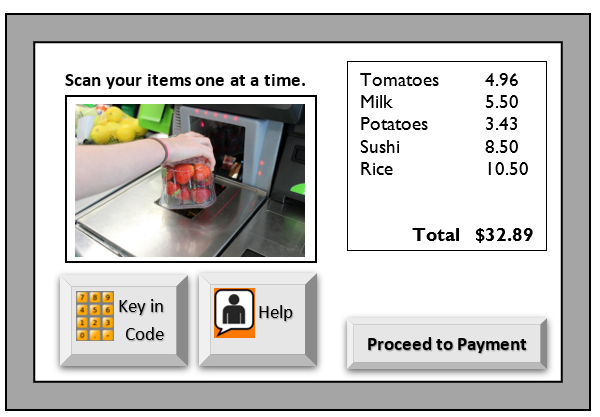
\includegraphics[width=0.5\paperwidth]{C:/Users/Admin/Desktop/Github/question_bank/LyX/static/img/9597-IJC-2018-P2-Q2-1}
\par\end{center}
\begin{enumerate}
\item State the type of user interface being used. \hfill{}{[}1{]}
\item Name \textbf{two} user input methods for the user interface. \hfill{}
{[}2{]}
\item Identify \textbf{one} feature of the user interface and explain the
design consideration involved in the choice of this feature. \hfill{}{[}3{]}
\end{enumerate}
\textquotedblleft Many people confuse the Internet as cloud computing\textquotedblright .
\begin{enumerate}
\item[(d)]  Explain how the Internet and cloud computing are different. \hfill{}{[}2{]}
\end{enumerate}
PriceFare intends to launch an online service in Singapore. Customers
can purchase their groceries using a mobile application anywhere in
Singapore. The management of PriceFare is deciding between two different
types of cloud services for this project -- Platform as a Service
(PaaS) and Infrastructure as a Service (IaaS). 
\begin{enumerate}
\item[(e)]  Describe the differences between PaaS and IaaS. \hfill{} {[}2{]}
\item[(f)]  What should the management of PriceFare consider when choosing between
these two types of cloud services? \hfill{}{[}2{]}
\item[(g)]  Give a reason why Software as a Service (SaaS) is not considered
by the management of PriceFare. \hfill{} {[}1{]}
\end{enumerate}